\documentclass[standalone, border=2mm]{standalone}
\usepackage{pgfplots}
\pgfplotsset{compat=1.18}

% Định nghĩa màu sắc (mã hex cho web)
% \definecolor{primary}{HTML}{2E86C1}   % Xanh dương hiện đại
\definecolor{primary}{HTML}{222B36}   % Xanh dương hiện đại
\definecolor{secondary}{HTML}{000000} % Cam
\definecolor{neutral}{HTML}{7F8C8D}   % Xám trung tính

\begin{document}
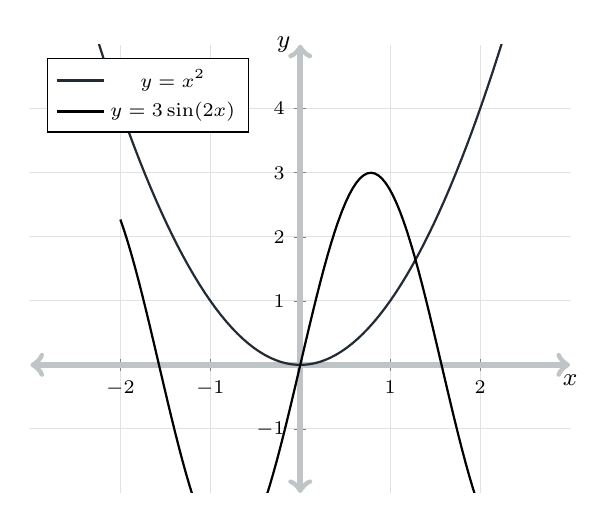
\begin{tikzpicture}
  \begin{axis}[
    font=\footnotesize\sf, % Phông chữ sans-serif nhỏ
    axis lines=middle,
    xlabel=$x$, ylabel=$y$,
    xmin=-3, xmax=3,
    ymin=-2, ymax=5,
    xtick={-2,-1,0,1,2},
    ytick={-1,0,1,2,3,4},
    grid=major,
    grid style={solid, neutral!25},
    axis line style={thin, <->, neutral!50, line width=2pt},
    tick label style={font=\scriptsize\sf},
    xlabel style={below, font=\small\sf},
    ylabel style={left, font=\small\sf},
    legend style={at={(0.03,0.97)}, anchor=north west, font=\scriptsize\sf},
  ]
  \addplot [
    domain=-3:3,
    samples=100,
    thick,
    color=primary,
  ]
  {x^2};
  \label{plot:x2}

  \addplot [
    domain=-2:2,
    samples=100,
    thick,
    color=secondary,
  ]
  {sin(deg(2*x)) * 3};
  \label{plot:sin}

  \legend{$y = x^2$, $y = 3\sin(2x)$};

  \end{axis}
\end{tikzpicture}
\end{document}